\subsection{BÀI TẬP TRẮC NGHIỆM}
\Opensolutionfile{ans}[ans/ansTL-0D2-B1]

\begin{ex}%[0D4B4]
	Bất phương trình nào sau đây là bất phương trình bậc nhất hai ẩn?
	\choice
	{$2x+y^3-z<3$}
	{$2x^2-2x+1\leq 0$}
	{$(x+y)(x-y)\geq 0$}
	{\True $3x-2y>1$}
	\loigiai{
	}
\end{ex}

\begin{ex}%[0D4B4]
	Trong các bất phương trình sau, bất phương trình nào \textbf{không phải} là bất phương trình bậc nhất hai ẩn?
	\choice{$2x+3y>0$}
	{\True $x+y^2 \leq 7$}
	{$x+2 \geq 0$}
	{$x-y>0$}
	\loigiai{
	}
\end{ex}

\begin{ex}%[0D4B4]
	Bất phương trình $x+2y\leq 3$ có bao nhiêu nghiệm?
	\choice
	{$1$}
	{$2$}
	{Vô nghiệm}
	{\True Vô số nghiệm}
	\loigiai{
	}
\end{ex}

\begin{ex}
	Miền nghiệm của bất phương trình $ax+by\leq c$ bỏ đi phần đường thẳng $ax+by=c$ được miền nghiệm của bất phương trình nào sau đây?
	\choice
	{$ax+by\geq c$}
	{$ax+by>c $}
	{\True $ax+by<c $}
	{$ ax+by>0$}
	\loigiai{
	}
\end{ex}

\begin{ex}%[0D4B4]
	Bất phương trình $ 5x-2(y-x+1)>0$ tương đương với bất phương trình nào sau đây?
	\choice
	{\True $7x-2y-2>0$}
	{$5x-2y>1$}
	{$5x-y-2>0$}
	{$3x-2y-2>0$}
	\loigiai{
		Xét $$ 5x-2(y-x+1)>0 \Leftrightarrow 5x -2y +2x -2 >0 \Leftrightarrow 7x-2y-2>0.$$
	}
\end{ex}

\begin{ex}%[0D4B4]
	Cặp số $(x;y)$ nào sau đây là một nghiệm của bất phương trình $2x+5y>10$?
	\choice
	{$(0;0)$}
	{$(2;-7)$}
	{$(-1;1) $}
	{\True $(2;5)$}
	\loigiai{
		Thử với $(2;5)$, ta có  $2 \cdot 2 + 5 \cdot 5 >10$ (đúng).\\ Vậy $(2;5)$ là nghiệm của bất phương trình $2x+5y>10$.
	}
\end{ex}

\begin{ex}%[Ngọc Hiếu]%[0D4Y4-1]%
	Cặp số $(x_0;y_0)$ nào là nghiệm của bất phương trình $2x-3y\geq 4$?
	\choice
	{$(x_0;y_0)=(2;1)$}
	{$(x_0;y_0)=(-2;2)$}
	{\True $(x_0;y_0)=(5;1)$}
	{$(x_0;y_0)=(-4;0)$}
	\loigiai{
		Nhận xét: Các phương án đưa ra đều có $y\geq 0$ nên ta biến đổi bất phương trình trên như sau:\\
		$2x-3y\geq 4\Leftrightarrow x\geq \dfrac{3y+4}{2}\Leftrightarrow x\geq \dfrac{3}{2}y + 2\Leftrightarrow x\geq 2, \forall y\geq 0$.\\
		Vậy cặp $(x_0;y_0)=(5;1)$ thỏa mãn.
	}
\end{ex}

\begin{ex}%[0D4B4]
	Cặp số nào sau đây {\bf không phải} là nghiệm của bất phương trình $3x+y\geq 4$ ?
	\choice
	{\True $(1;0)$}
	{$(1;1)$}
	{$(1;2)$}
	{$(4;1)$}
	\loigiai{
		Thử với $(1;0)$, ta có  $3 \cdot 1 + 0 >4$ (sai).\\ Vậy $(1;0)$ không là nghiệm của bất phương trình $3x+y\geq 4$.
	}
\end{ex}

\begin{ex}%[0D4Y4-1]%
	Điểm $A(-1;3)$ thuộc miền của bất phương trình
	\choice
	{$x+3y<0$}
	{$3x-y>0$}
	{\True  $-3x+2y-4>0$}
	{$2x-y+4>0$}
	\loigiai{
		Thay tọa độ $A(-1;3)$ vào các bất phương trình:
		\begin{itemize}
			\item[•] Với bất phương trình $x+3y<0$, ta có $(-1)+3\cdot 3<0$ sai.
			\item[•] Với bất phương trình $3x-y>0$, ta có $3\cdot (-1)-3>0$ sai.
			\item[•] Với bất phương trình $-3x+2y-4>0$, ta có $-3\cdot (-1)+2\cdot 3-4>0$ đúng.
			\item[•] Với bất phương trình $2x-y+4>0$, ta có $2\cdot (-1)-3+4>0$ sai.
		\end{itemize}
		Vậy $A(-1;3)$ thuộc miền nghiệm bất phương trình $-3x+2y-4>0$.
	}
\end{ex}

\begin{ex}%[Đề thi HKI khối 10 năm học 2019-2020]%[0D4Y4-1]%
	Cặp số $(-1;4)$ là nghiệm của bất phương trình
	\choice
	{$x-y+2>0$}
	{$-2x+y+1<0$}
	{\True $x+y+2>0$}
	{$x+y+4 \leq 0$}
	\loigiai{
		Thế$ x=-1$ và $y=4$ vào từng bất phương trìnhta thấy chỉ có thỏa mãn bất phương trình $x+y+2>0$.}
\end{ex}

\begin{ex}%[Nguyễn Trung Hiếu]%[781-810 Phạm Quốc Toàn]%[0D4K4-1]%
	Tìm tất cả các số thực $a$ sao cho miền nghiệm của bất phương trình $x\le a$ chứa điểm $M(-1;0)$.
	\choice
	{$a>-1$}
	{\True $a \ge -1$}
	{$a>0$}
	{$a\ge 0$}
	\loigiai{Để $M(-1;0)$ thuộc miền nghiệm của bất phương trình $x\le a$ thì $a \geq -1$.
	}
\end{ex}

\begin{ex}%[0D4K4-1]%
	Với giá trị nào của $m$ thì điểm $A(1-m;m)$ {\bf không thuộc} miền nghiệm của bất phương trình $2x-3(y-x)>4$.
	\choice
	{\True $m \geq \dfrac{1}{8}$}
	{$0\leq m \leq 1$}
	{$m<\dfrac{1}{8}$}
	{$\dfrac{1}{8}\leq m\leq 1$}
	\loigiai{
		$A(1-m;m)$ không thuộc miền nghiệm của bất phương trình $2x-3(y-x)>4$ khi tọa độ của nó không thỏa mãn bất phương trình, tức là $2(1-m)-3(m+m-1) \leq 4$ hay $m \geq \dfrac{1}{8}$.}
\end{ex}

\begin{ex}
	\immini[thm]{	
		Hình vẽ sau có phần không tô và cả trục $Oy$ là miền nghiệm của một trong bốn bất phương trình dưới đây. Hãy tìm bất phương trình đó. 
		\haicot
		{$x\geq 0$}
		{\True $x\leq 0$}
		{$y\geq 0$}
		{$y\leq 0$}}
	{		\begin{tikzpicture}[scale=.7,thick,>=stealth']
			\draw[->] (-2,0) -- (4.3,0)node[above]{$x$};
			\foreach \x in {-1,1,2,3,4}
			\draw[shift={(\x,0)},color=black] (0pt,2pt) -- (0pt,-2pt) node[below] {\footnotesize $\x$};
			\draw[->,color=black] (0,-1) -- (0,4)node[left]{$y$};
			\foreach \y in {1,2,3}
			\draw[shift={(0,\y)},color=black] (2pt,0pt) -- (-2pt,0pt) node[left] {\footnotesize $\y$};
			\node[above left] at (0,0){$O$};
			\fill[pattern=north east lines,pattern color=myblue] (0,-1) -- (4,-1) -- (4,4) -- (0,4) -- cycle;
		\end{tikzpicture}
	}
	\loigiai{
	}
\end{ex}

\begin{ex}
	\immini[thm]{Hãy chọn bất phương trình mà miền nghiệm của nó là nửa mặt phẳng không bị gạch có bờ là đường thẳng $d$ như hình bên.
		\choice
		{$x-y>4$}
		{$x-y<4$}
		{$x-y\le 4$}
		{\True $x-y\ge 4$}
	}
	{
		\begin{tikzpicture}[>=stealth',scale=0.6]
			\def\xmin{-2} \def\xmax{5}
			\def\ymin{-5} \def\ymax{2}
			\tkzDefPoints{\xmax/\ymax/A1,\xmin/\ymax/A2,\xmin/\ymin/A3,\xmax/\ymin/A4}
			\tkzDefPoints{5/1/M,-1/-5/N, 4/0/A,0/-4/B}
			\fill[pattern=north west lines,pattern color=myblue] (M)--(A1)--(A2)--(A3)--(N)--cycle;
			\tkzDrawPoints(A,B)
			\draw[domain=-1:5] plot(\x,{(\x)-4});
			\begin{scriptsize}
				\draw[->](\xmin,0)--(\xmax,0); \draw(\xmax-0.1,0) node[below]{$x$};
				\draw[->](0,\ymin)--(0,\ymax); \draw(0,\ymax-0.2) node[right]{$y$};
				\draw node [above right]{$O$} 
				(A) node [below]{$4$} 
				(B) node [right]{$-4$}
				(2,-2) node [below]{$d$};
			\end{scriptsize}
		\end{tikzpicture}
	}
	\loigiai{
		\begin{itemize}
			\item [$\bullet$] Ta có $(5;0)$ thuộc miền nghiệm của bất phương trình, nhưng tọa độ điểm này lại không thỏa phương án B và C, suy ra phương án B và C bị loại.
			\item [$\bullet$] Do miền nghiệm lấy cả phần đường thẳng (có dấu bằng) nên ta chọn phương án D.
		\end{itemize}
	}
\end{ex}

\begin{ex}%[0D4K4-1]%
	\immini[thm]{ Phần không bị gạch trong hình vẽ sau, biểu diễn tập nghiệm của bất phương trình nào trong các bất phương trình sau?
		\haicot
		{$x-2y<3$}
		{\True $2x-y>3$}
		{$x-2y>3$}
		{$2x-y<3$}
	}
	{
		\begin{tikzpicture}[scale=0.7, font=\footnotesize, line join=round, line cap=round, >=stealth]
			\def\xmin{-1}\def\xmax{3.0}\def\ymin{-4.0}\def\ymax{1}
			\draw[->] (\xmin-0.2,0)--(\xmax+0.2,0) node[below] {\footnotesize $x$};
			\draw[->] (0,\ymin)--(0,\ymax+0.2) node[right] {$y$};
			\draw (0,0) node [below left] {$O$};
			\foreach \x in {1,2}\draw (\x,0.1)--(\x,-0.1) node [below] {\footnotesize $\x$};
			\foreach \y in {-3}\draw (0.1,\y)--(-0.1,\y) node [left] {\footnotesize $\y$};
			\draw[smooth,samples=200,domain=-0.5:2] plot (\x,{2*(\x)-3});
			\fill[pattern=north east lines,pattern color=myblue] (-0.5,-4) -- (-1,-4) -- (-1,1) -- (2,1) -- cycle;
		\end{tikzpicture}
	}
	\loigiai{
		Đường thẳng đi qua $A\left(\dfrac{3}{2};0\right)$ và $B(0;-3)$ nên có phương trình $2x-y=3$.\\
		Mặt khác, cặp số $(0;0)$ không thỏa mãn bất phương trình $2x-y>3$ nên phần tô đậm ở hình trên là miền nghiệm bất phương trình $2x-y>3$.
	}
\end{ex}

\begin{ex}%[0D4B4-1]%
	Miền nghiệm của bất phương trình $3x-2y<-6$ (phần không bị gạch) được biểu diễn bởi hình nào sau đây?
	\choice
	{\begin{tikzpicture}[scale=0.6,>=stealth]
			%---------------------- Vẽ hệ trục tọa độ
			\draw[->] (-3.25,0)--(3.25,0) node[below right] {$x$};
			\draw[->] (0,-1)--(0,3.6) node[right] {$y$};
			\node (0,0) [above right]{$ O $};
			%----------------------- Vẽ đoạn chắn trên trục
			\foreach \x in {-3,-2,-1,1,2,3}
			\draw[shift={(\x,0)},color=black] (0pt,2pt) -- (0pt,-2pt);
			%\node at (3.8,0.5) {$4$};
			\foreach \y in {1,2,3}
			\draw[shift={(0,\y)},color=black] (2pt,0pt) -- (-2pt,0pt);
			\node at (2.3,0.3) {$2$};
			\node at (-0.3,3) {$3$};
			%--------------------- Vẽ hàm
			\draw [thick, domain=-0.4:2.67, samples=100] plot (\x, {-(3/2)*\x +3});
			%----------------------Vẽ miền nghiệm
			\tkzDefPoints{-0.4/3.6/A, -3.25/3.6/B, -3.25/-1/C, 2.67/-1/D}
			\tkzDrawPolygon[pattern=north east lines,opacity=.5,pattern color=myblue](A,B,C,D)
	\end{tikzpicture}}
	{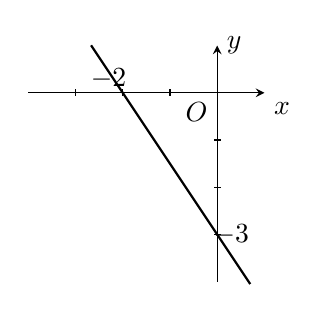
\begin{tikzpicture}[scale=0.6,>=stealth]
			%---------------------- Vẽ hệ trục tọa độ
			\draw[->] (-4,0)--(1,0) node[below right] {$x$};
			\draw[->] (0,-4)--(0,1) node[right] {$y$};
			\node (0,0) [below left]{$ O $};
			%----------------------- Vẽ đoạn chắn trên trục
			\foreach \x in {-3,-2,-1}
			\draw[shift={(\x,0)},color=black] (0pt,2pt) -- (0pt,-2pt);
			\foreach \y in {-3,-2,-1}
			\draw[shift={(0,\y)},color=black] (2pt,0pt) -- (-2pt,0pt);
			\node at (-2.3,0.3) {$-2$};
			\node at (0.3,-3) {$-3$};
			%--------------------- Vẽ hàm
			\draw [thick, domain=-2.67:0.7, samples=100] plot (\x, {-(3/2)*\x -3});
			%----------------------Vẽ miền nghiệm
			\tkzDefPoints{-2.67/1/A, -4/1/B, -4/-4/C, 0.66/-4/D}
			\tkzDrawPolygon[ pattern=north east lines,opacity=.5,pattern color=myblue](A,B,C,D)
	\end{tikzpicture}}
	{\True \begin{tikzpicture}[scale=0.6,>=stealth]
			\draw[->] (-3.25,0)--(3.25,0) node[below right] {$x$};
			\draw[->] (0,-1)--(0,3.6) node[right] {$y$};
			\node (0,0) [above right]{$ O $};
			\foreach \x in {-1,1,2,3}
			\draw[shift={(\x,0)},color=black] (0pt,2pt) -- (0pt,-2pt);
			%\node at (3.8,0.5) {$4$};
			\foreach \y in {-1,1,2,3}
			\draw[shift={(0,\y)},color=black] (2pt,0pt) -- (-2pt,0pt);
			\node at (-2.3,0.3) {$-2$};
			\node at (-0.3,3) {$3$};
			%--------------------- Vẽ hàm
			\draw [domain=-2.67:0.4, samples=100] plot (\x, {(3/2)*\x +3});
			\tkzDefPoints{0.4/3.6/A, 3/3.6/B, 3/-1/C, -2.67/-1/D}
			\tkzDrawPolygon[pattern=north east lines,opacity=0.5,pattern color=myblue](A,B,C,D)
	\end{tikzpicture}}
	{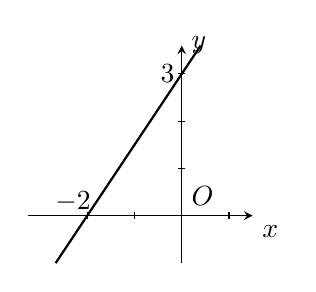
\begin{tikzpicture}[scale=0.6,>=stealth]
			%---------------------- Vẽ hệ trục tọa độ
			\draw[->] (-3.25,0)--(1.5,0) node[below right] {$x$};
			\draw[->] (0,-1)--(0,3.6) node[right] {$y$};
			\node (0,0) [above right]{$ O $};
			%----------------------- Vẽ đoạn chắn trên trục
			\foreach \x in {-2,-1,1}
			\draw[shift={(\x,0)},color=black] (0pt,2pt) -- (0pt,-2pt);
			\foreach \y in {1,2,3}
			\draw[shift={(0,\y)},color=black] (2pt,0pt) -- (-2pt,0pt);
			\node at (-2.3,0.3) {$-2$};
			\node at (-0.3,3) {$3$};
			%--------------------- Vẽ hàm
			\draw [thick, domain=-2.67:0.4, samples=100] plot (\x, {(3/2)*\x +3});
			%----------------------Vẽ miền nghiệm
			\tkzDefPoints{0.4/3.6/A, -3.25/3.6/B, -3.25/-1/C, -2.67/-1/D}
			\tkzDrawPolygon[ pattern=north east lines,opacity=.5,pattern color=myblue](A,B,C,D)
	\end{tikzpicture}}
	\loigiai{
		Ta thấy $O(0;0)$ không thuộc miền nghiệm của bất phương trình nên loại A và B.
		Xét điểm $M(-2;3)$ không thuộc miền nghiệm của bất phương trình nên loại D.
}
\end{ex}

\begin{ex}%[BG Toán 10-2022]%[Trần Nhân Kiệt]%[0D4T4-3]
	Trong $1$ lạng ($100$ g) thịt bò chứa khoảng $26$ g protein và $1$ lạng cá rô phi chứa khoảng $20$ g protein. Trung bình trong một ngày, một người đàn ông cần tối thiểu $52$ g protein. Gọi $x$, $y$ lần lượt là số lạng thịt bò và số lạng cá rô phi mà một người đàn ông nên ăn trong một ngày. Viết bất phương trình bậc nhất hai ẩn $x$, $y$ để biểu diễn lượng protein cần thiết cho một người đàn ông trong một ngày.
	\choice
	{$26x+20y\le 52$}
	{$26x+20y< 52$}
	{\True $13x+10y\ge 26$}
	{$13x+10y> 26$}
	\loigiai{
		Trong $x$ lạng thịt bò chứa $26x$ g protein.\\
		Trong $y$ lạng cá rô phi chứa $20y$ g protein.\\
		Do đó lượng protein cần thiết trong một ngày của một người đàn ông là 
		$$26x+20y\ge 52\Leftrightarrow 13x+10y\ge 26.$$
	}
\end{ex}

\begin{ex}%[BG Toán 10-2022]%[Trần Nhân Kiệt]%[0D4T4-3]
	Công ty viễn thông Viettel có gói cước Hi School tính phí là $1190$ đồng mỗi phút gọi nội mạng và $1390$ đồng mỗi phút gọi ngoại mạng. Một bạn học sinh đăng kí gói cước trên và sử dụng $x$ phút gọi nội mạng, $y$ phút gọi ngoại mạng trong một tháng. Viết bất phương trình bậc nhất hai ẩn $x$, $y$ để mô tả số tiền bạn đó phải trả trong một tháng ít hơn $100$ nghìn đồng.
	\choice
	{$119x+139y\ge 10000$}
	{$139x+119y< 10000$}
	{$119x+139y\le 10000$}
	{\True $119x+139y< 10000$}
	\loigiai{
		Trong một tháng, số tiền gọi nội mạng là $1190 x$ đồng và số tiền gọi ngoại mạng là $1390y$ đồng.\\
		Tổng số tiền trong một tháng bạn học sinh phải trả là $1190x+1390y$.\\
		Để số tiền trong một tháng phải trả ít hơn $100$ nghìn đồng thì 
		$$1190x+1390y< 100000\Leftrightarrow 119y+139y< 10000.$$
		
	}
\end{ex}

\begin{ex}%[BG Toán 10-2022]%[Trần Nhân Kiệt]%[0D4T4-3]
	Ngoài giờ học, bạn Nam làm thêm việc phụ bán cơm được $15$ nghìn đồng/một giờ và phụ bán tạp hóa được $10$ nghìn đồng/một giờ. Gọi $x$, $y$ lần lượt là số giờ phụ bán cơm và phụ bán tạp hóa trong mỗi tuần. Viết bất phương trình bậc nhất hai ẩn $x$ và $y$ sao cho Nam kiếm thêm tiền mỗi tuần được ít nhất là $900$ nghìn đồng.
	\choice
	{$3x+2y\le 180$}
	{$3x+2y> 180$}
	{\True $3x+2y\ge 180$}
	{$3x+2y< 180$}
	\loigiai{
		Số tiền từ việc phụ bán cơm là $15x$ nghìn đồng và số tiền từ việc phụ bán tạp hóa là $10y$ nghìn đồng.\\
		Số tiền Nam kiếm được mỗi tuần là $15x+10y$.\\
		Để số tiền Nam kiếm được mỗi tuần ít nhất là $900$ nghìn đồng thì 
		$$15x+10y\ge 900\Leftrightarrow 3x+2y\ge 180.$$
	}
\end{ex}
\begin{ex}%[BG Toán 10-2022]%[Trần Nhân Kiệt]%[0D4T4-3]
	Anh A muốn thuê một chiếc ô tô (có người lái) trong một tuần. Giá thuê xe như sau: từ thứ hai đến thứ sáu phí cố định là $900$ nghìn đồng/ngày và phí tính theo quãng đường di chuyển là $10$ nghìn đồng/km còn thứ bảy và chủ nhật thì phí cố định là $1200$ nghìn đồng/ngày và phí tính theo quãng đường di chuyển là $15$ nghìn đồng/km. Gọi $x$, $y$ lần lượt là số km mà anh A đi trong các ngày từ thứ hai đến thứ sáu và trong hai ngày cuối tuần. Viết bất phương trình biểu thị mối liên hệ giữa $x$ và $y$ sao cho tổng số tiền anh A phải trả không quá $20$ triệu đồng.
	\choice
	{$10x+15y\le 20000$}
	{$2x+3y\ge 2720$}
	{$10x+15y\ge 20000$}
	{\True $2x+3y\le 2720$}
	\loigiai{
		Số tiền thuê xe của anh A từ thứ hai đến thứ sáu là $900\cdot 5+10x$ nghìn đồng và hai ngày thứ bảy, chủ nhật là $1200\cdot 2+15y$ nghìn đồng.\\
		Để số tiền anh A phải trả không quá $20$ triệu đồng thì 
		$$(900\cdot 5+10x)+(1200\cdot 2+15y)\le 20000\Leftrightarrow 2x+3y\le 2720.$$
	}
\end{ex}
%\centerline{\textbf{---HẾT---}}
\Closesolutionfile{ans}